\documentclass{article}
    \usepackage{caption}
    \usepackage{subcaption}
    \usepackage{mathtools}
    \usepackage{algorithm2e}
    
    \usepackage{enumerate}% section item
    \usepackage{amssymb}  % \varnothing
    \usepackage{booktabs} % insert table
    \usepackage{multirow} % table combine
    \usepackage{listings} % insert code
    \usepackage{appendix} % 
    \usepackage{amsmath}  % for mathfont
    \usepackage{unicode-math} % for mathfont
    \usepackage{fontspec} % set font
    \setmainfont{Times} % main font
    \newfontfamily\monaco{Monaco} % code font
    \usepackage{pythonhighlight} % python
   % \usepackage{hyperref}

    \usepackage{listings}
    \usepackage{color}
    \usepackage{xcolor}
    \definecolor{dkgreen}{rgb}{0,0.6,0}
    \definecolor{gray}{rgb}{0.5,0.5,0.5}
    \definecolor{mauve}{rgb}{0.58,0,0.82}
    \lstset{frame=tb,
        language=Java,
        aboveskip=3mm,
        belowskip=3mm,
        showstringspaces=false,
        columns=flexible,
        basicstyle = \ttfamily\small,
        numbers=none,
        numberstyle=\tiny\color{gray},
        keywordstyle=\color{blue},
        commentstyle=\color{dkgreen},
        stringstyle=\color{mauve},
        breaklines=true,
        breakatwhitespace=true,
        tabsize=3
    }


    \usepackage[colorlinks=true]{hyperref} % the option is there to remove the square around links which is what I don't like.
    
    \usepackage{perpage} 
    \MakePerPage{footnote} % Reset the footnote counter perpage. may require to run latex twice.
    
    \usepackage[margin=2cm]{geometry} % This is here to fit more text into the page.
    
 %   \setcounter{secnumdepth}{1}  % This removes the numbering from the subsections.
                            % If you want the numbering of the subsection level just remove this line
    
    \title{\textsc{COMP7506 - CourseSchedule}}
    \author{	Group - 14 \\
                3035562502 - ZHANG Kai \\
                3035562100 - WANG Dezhao \\
                3035562069 - YAN Qiangyu }
    \date{}
    
    \setlength{\parindent}{0pt} % No indentation for paragraphs. Because that is just old.
    \setlength{\parskip}{\baselineskip} % Instead use vertical paragraph spacing.
    
    %\setmainfont{Helvetical} % Setting the main font here. But I like the default font alot so this is commented out.
    
    \begin{document}
    \maketitle
    
    
    \section{Background Research}

    \subsection{Category \& Function Synopsis}
    CourseSchedule is an eduactional Andriod application that aims to 
    make students get their course schedule easier.
    
    In this App, students can get their course schedule
    once they logged in with right portal account, 
    and it's the mian function of this App.
    With this App, users can view their course with different colors.
    Meanwhile, this App also provides the function

    \subsection{Market Analysis}

    \subsection{Similar Apps}
    \subsubsection{QSC}
    \begin{center}
        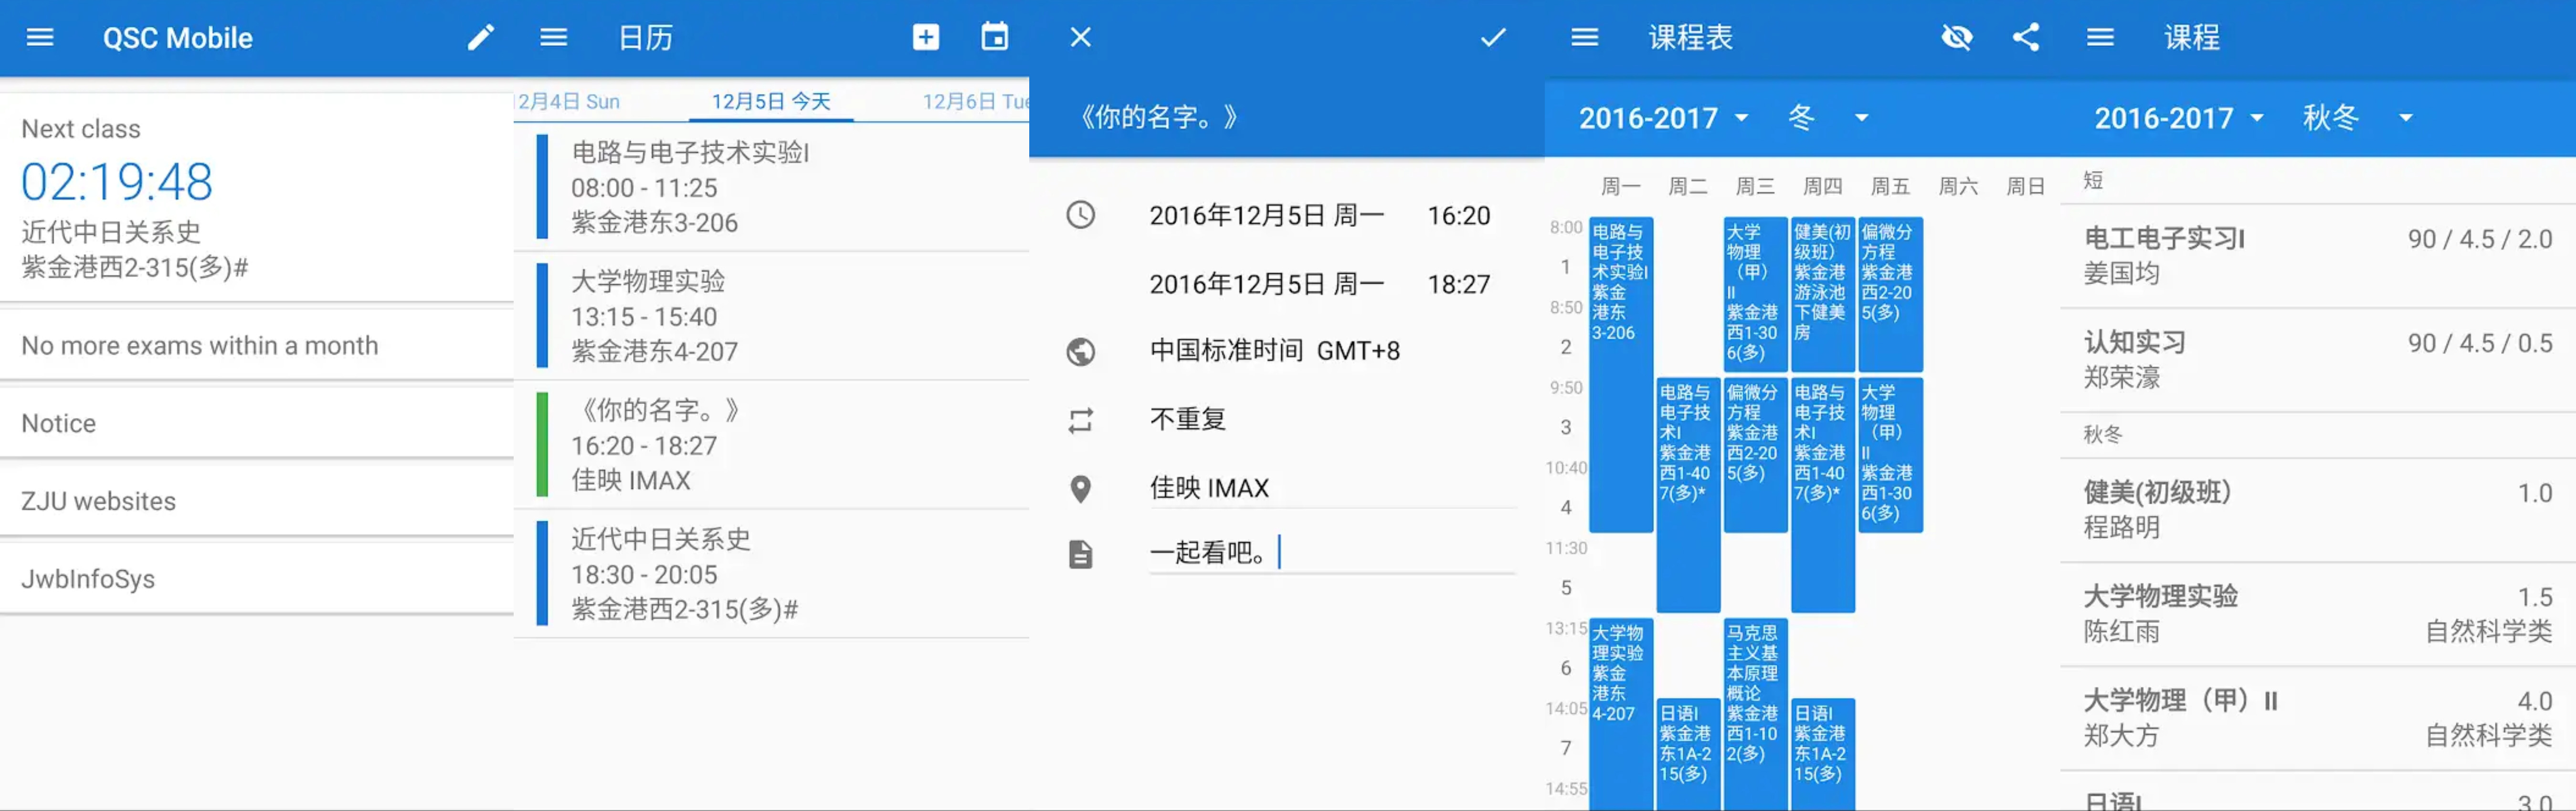
\includegraphics[width=6.9in]{QSC}
    \end{center}
    \begin{enumerate}[i)]
        \item Overview
        \item short-comings / possible improvements
    \end{enumerate}
    

    \subsubsection{CourseGrid}
    \begin{center}
        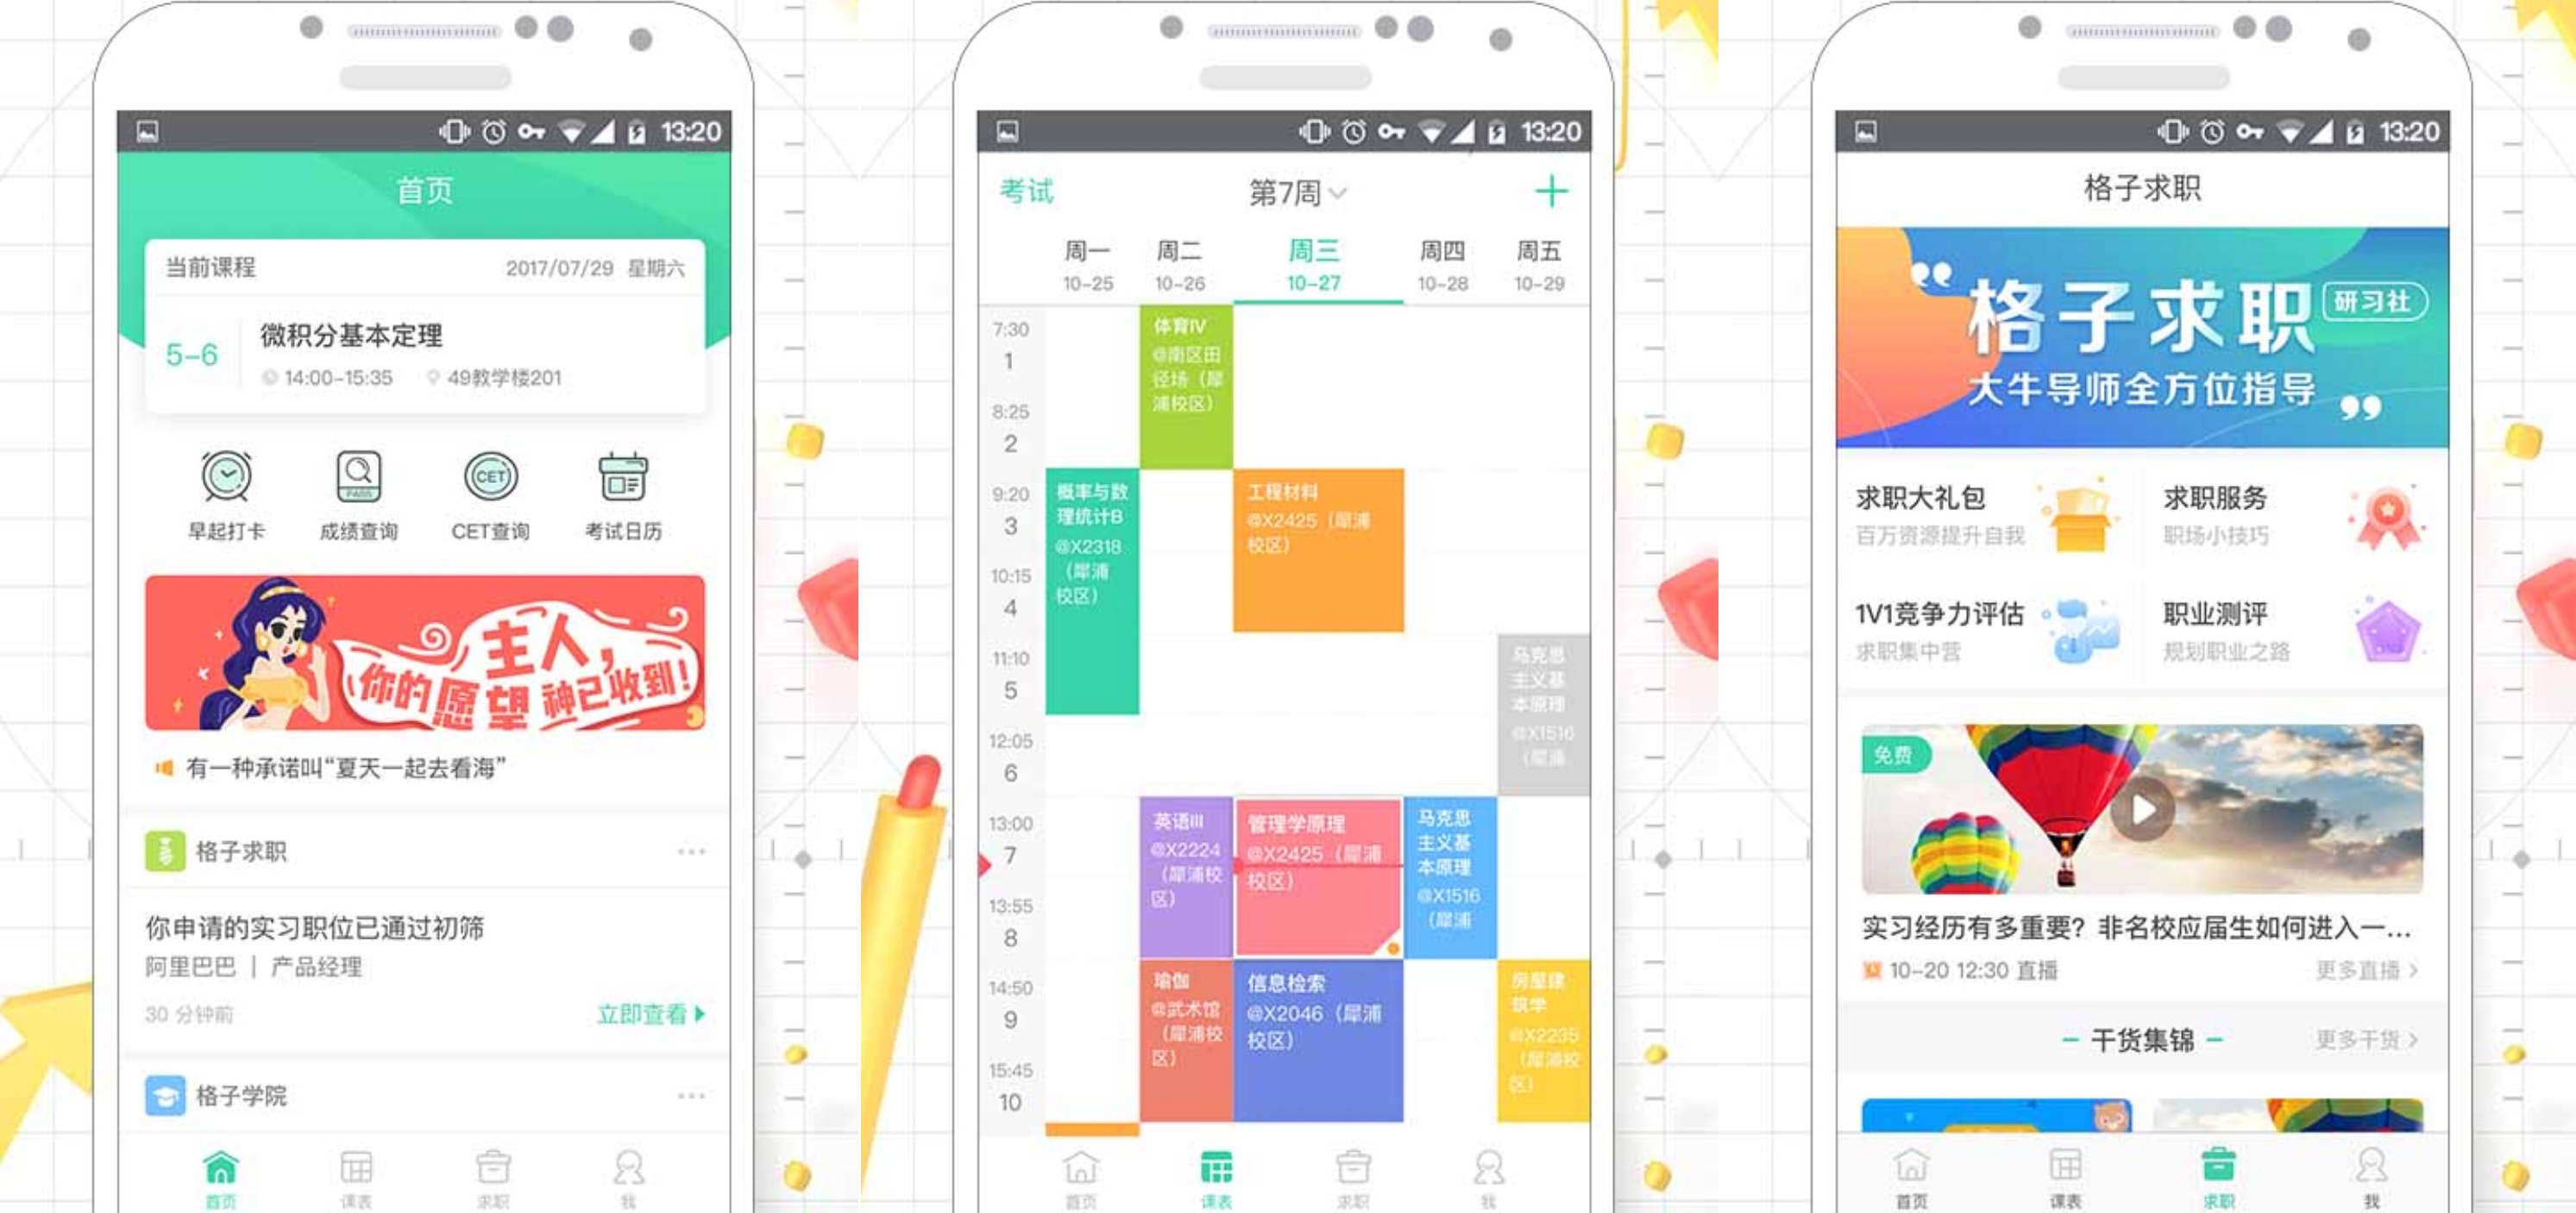
\includegraphics[width=6.5in]{CourseGrid}
    \end{center}

    \subsubsection{SuperCurriculum}
    \begin{center}
        
\includegraphics[width=6.5in]{SuperCurriculum}
    \end{center}

    \section{Main functions}

    \begin{enumerate}[a)]
    \item MainActivity.java
    
    The app starts with this activity and 
    set content view to activity\_main.xml.

    \begin{lstlisting}[ language=Java]
private void initNavigationView():
    \end{lstlisting}
    Initialize the menu data in expandableListView and populate the expandable list. Set adapter, setOnGroupClickListener and setOnChildClickListener here.

    
    \end{enumerate}
    
 


    
    \section{Contributions}

    \begin{table}[h]
        \centering
        \begin{tabular}{|c|l|}
            \hline
            \multirow{7}{*}{ZHANG Kai} &  Main activity with layout/main.xml\\
            \cline{2-2}
            &Switch fragment functions \\
            \cline{2-2}
            &Fragment of homepage, corresponding layout xml file \\
            \cline{2-2}
            &Toolbar function and xml, bind toggle icon with drawer listener \\
            \cline{2-2}
            & Custom HolderView implements Holder, 
            implement automatic scrolling of pictures with\\
            & ConvenientBann\\
            \cline{2-2}
            &Complete the draft documentation, and Readme.md \\
            \hline
            \multirow{7}{*}{WANG Dezhao} &  
            Fragment of basic info (fees, overview, schedule), 
            corresponding layout xml files\\
            \cline{2-2}
            & Fragment of about (faculty, about HKU), 
            corresponding layout xml files \\
            \cline{2-2}
            & Custom ExpandableListAdapter and MenuModel item, 
            with list\_group\_child.xml/ \\
            & list\_group\_header.xml,
             generate custom drawer controls \\
            \cline{2-2}
            & View pager function, custom pager adapter \\
            \cline{2-2}
            & Page view layout files including Programme Overview, 
            Stream of Study, Selection of Courses, \\
            & Dissertations \\
            \hline
            \multirow{7}{*}{YAN Qiangyu} &  
            Fragment of news \& events, corresponding layout xml files\\
            \cline{2-2}
            & Custom loading view \\
            \cline{2-2}
            & Custom card view of news and card view of events \\
            \cline{2-2}
            & Multi-threaded operation when using Jsoup 
            to scratch message from URL and parse HTML \\
            \cline{2-2}
            & Update UI by using UIThread \\
            \cline{2-2}
            & Make the video \\
            \cline{2-2}
            & Review and complete the final documentation \\
            \hline
        \end{tabular}
    \end{table}

    \end{document}